\begin{figure}[!htb]
\centering
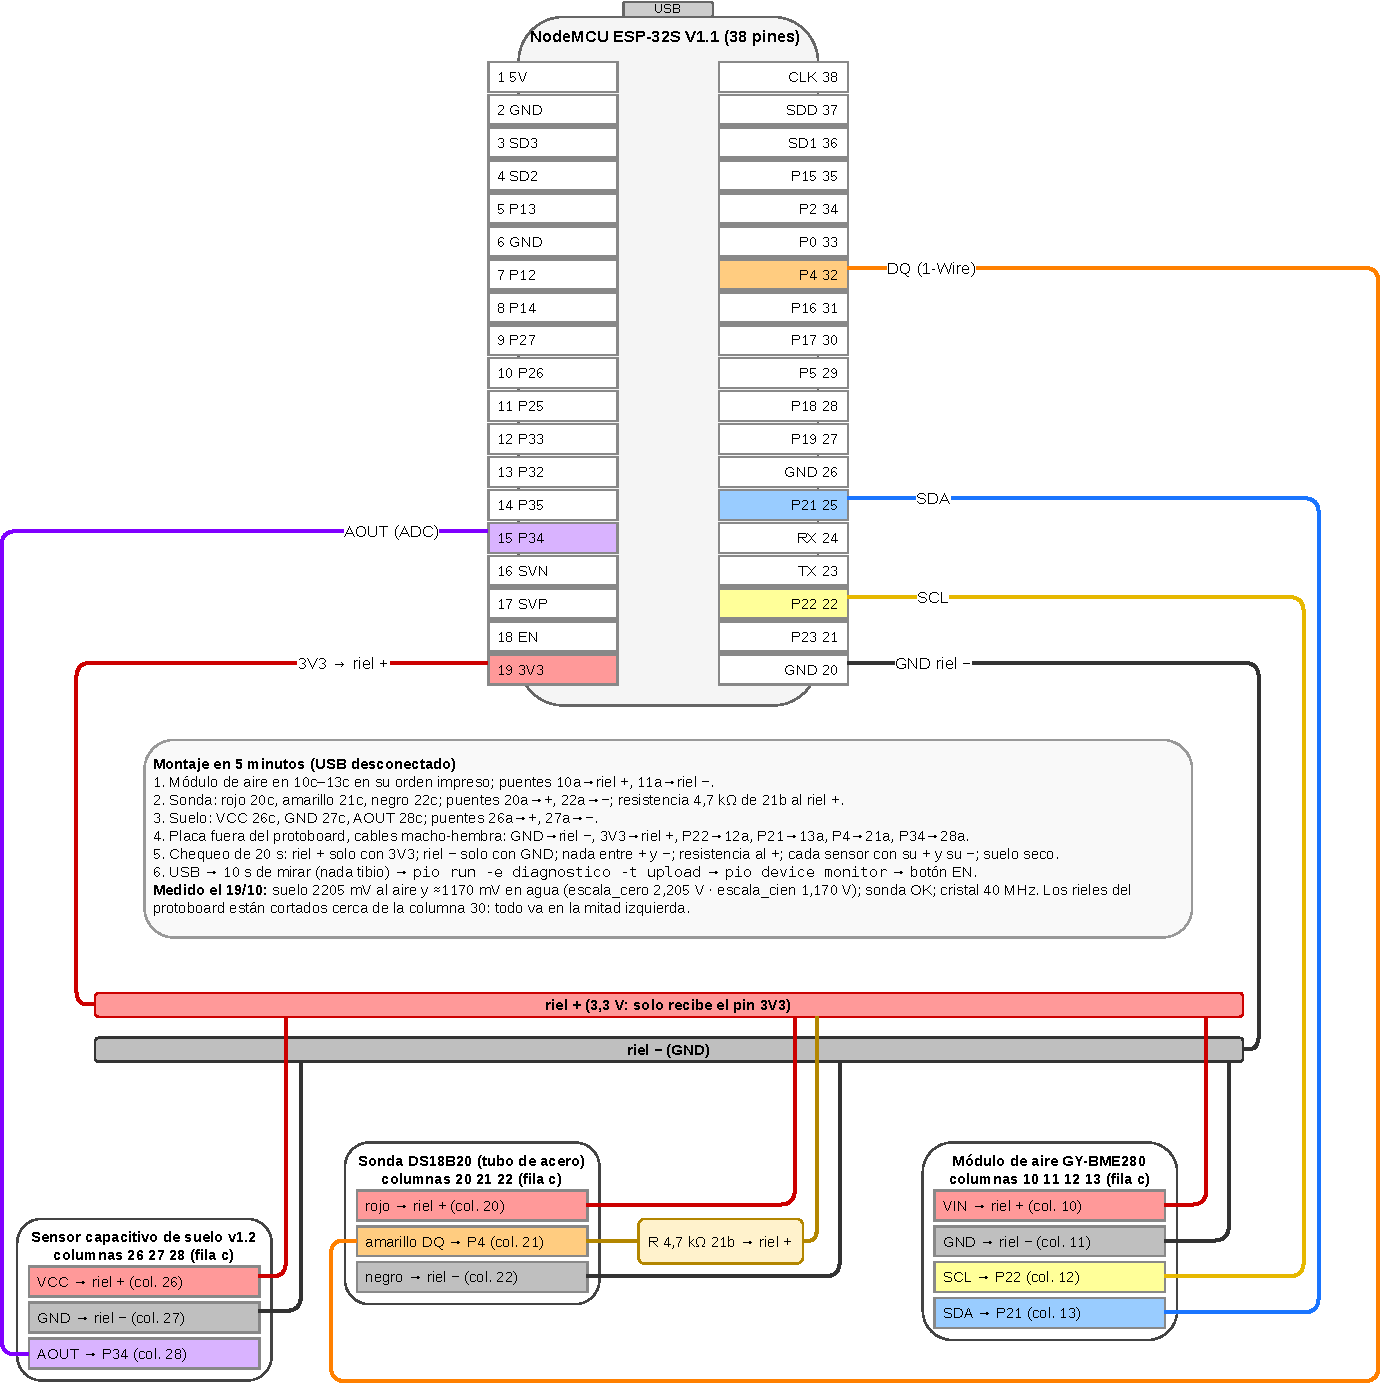
\includegraphics[width=\linewidth,height=0.78\textheight,keepaspectratio]{presentacion/figuras/cableado-esp32.pdf}
\caption[Cableado del nodo propio (fase 1)]{Cableado del nodo propio (fase 1, verificado el 19 de octubre de 2026): placa NodeMCU ESP-32S de 38 pines con el módulo de aire BME280 (I2C: SDA en P21, SCL en P22), la sonda de temperatura DS18B20 en tubo de acero (1-Wire en P4, con resistencia de 4,7~k$\Omega$ al riel de 3,3~V) y el sensor capacitivo de humedad de suelo (analógico en P34), sobre una protoboard cuyos rieles reciben solo 3,3~V y tierra desde la placa. Se cablea sin corriente y se revisa antes de conectar el USB; los pines están verificados contra el firmware. Dibujo del autor (\texttt{plataforma/firmware/cableado-fase-1.drawio}); montaje, calibración y compra en \texttt{docs/17}.}
\label{fig:cableado}
\end{figure}
